\documentclass{article}
\usepackage[a4paper, margin=0.5in]{geometry}
\usepackage[utf8]{inputenc}
\usepackage{amsmath}
\usepackage{stmaryrd}
\usepackage{graphicx}

\renewcommand\t[1]{\text{#1}}
\renewcommand\d{\text{ . }}
\newcommand\lwt[1]{$_\text{#1}$}

\usepackage{graphicx}

\begin{document}

% \maketitle

\section{}


\centering
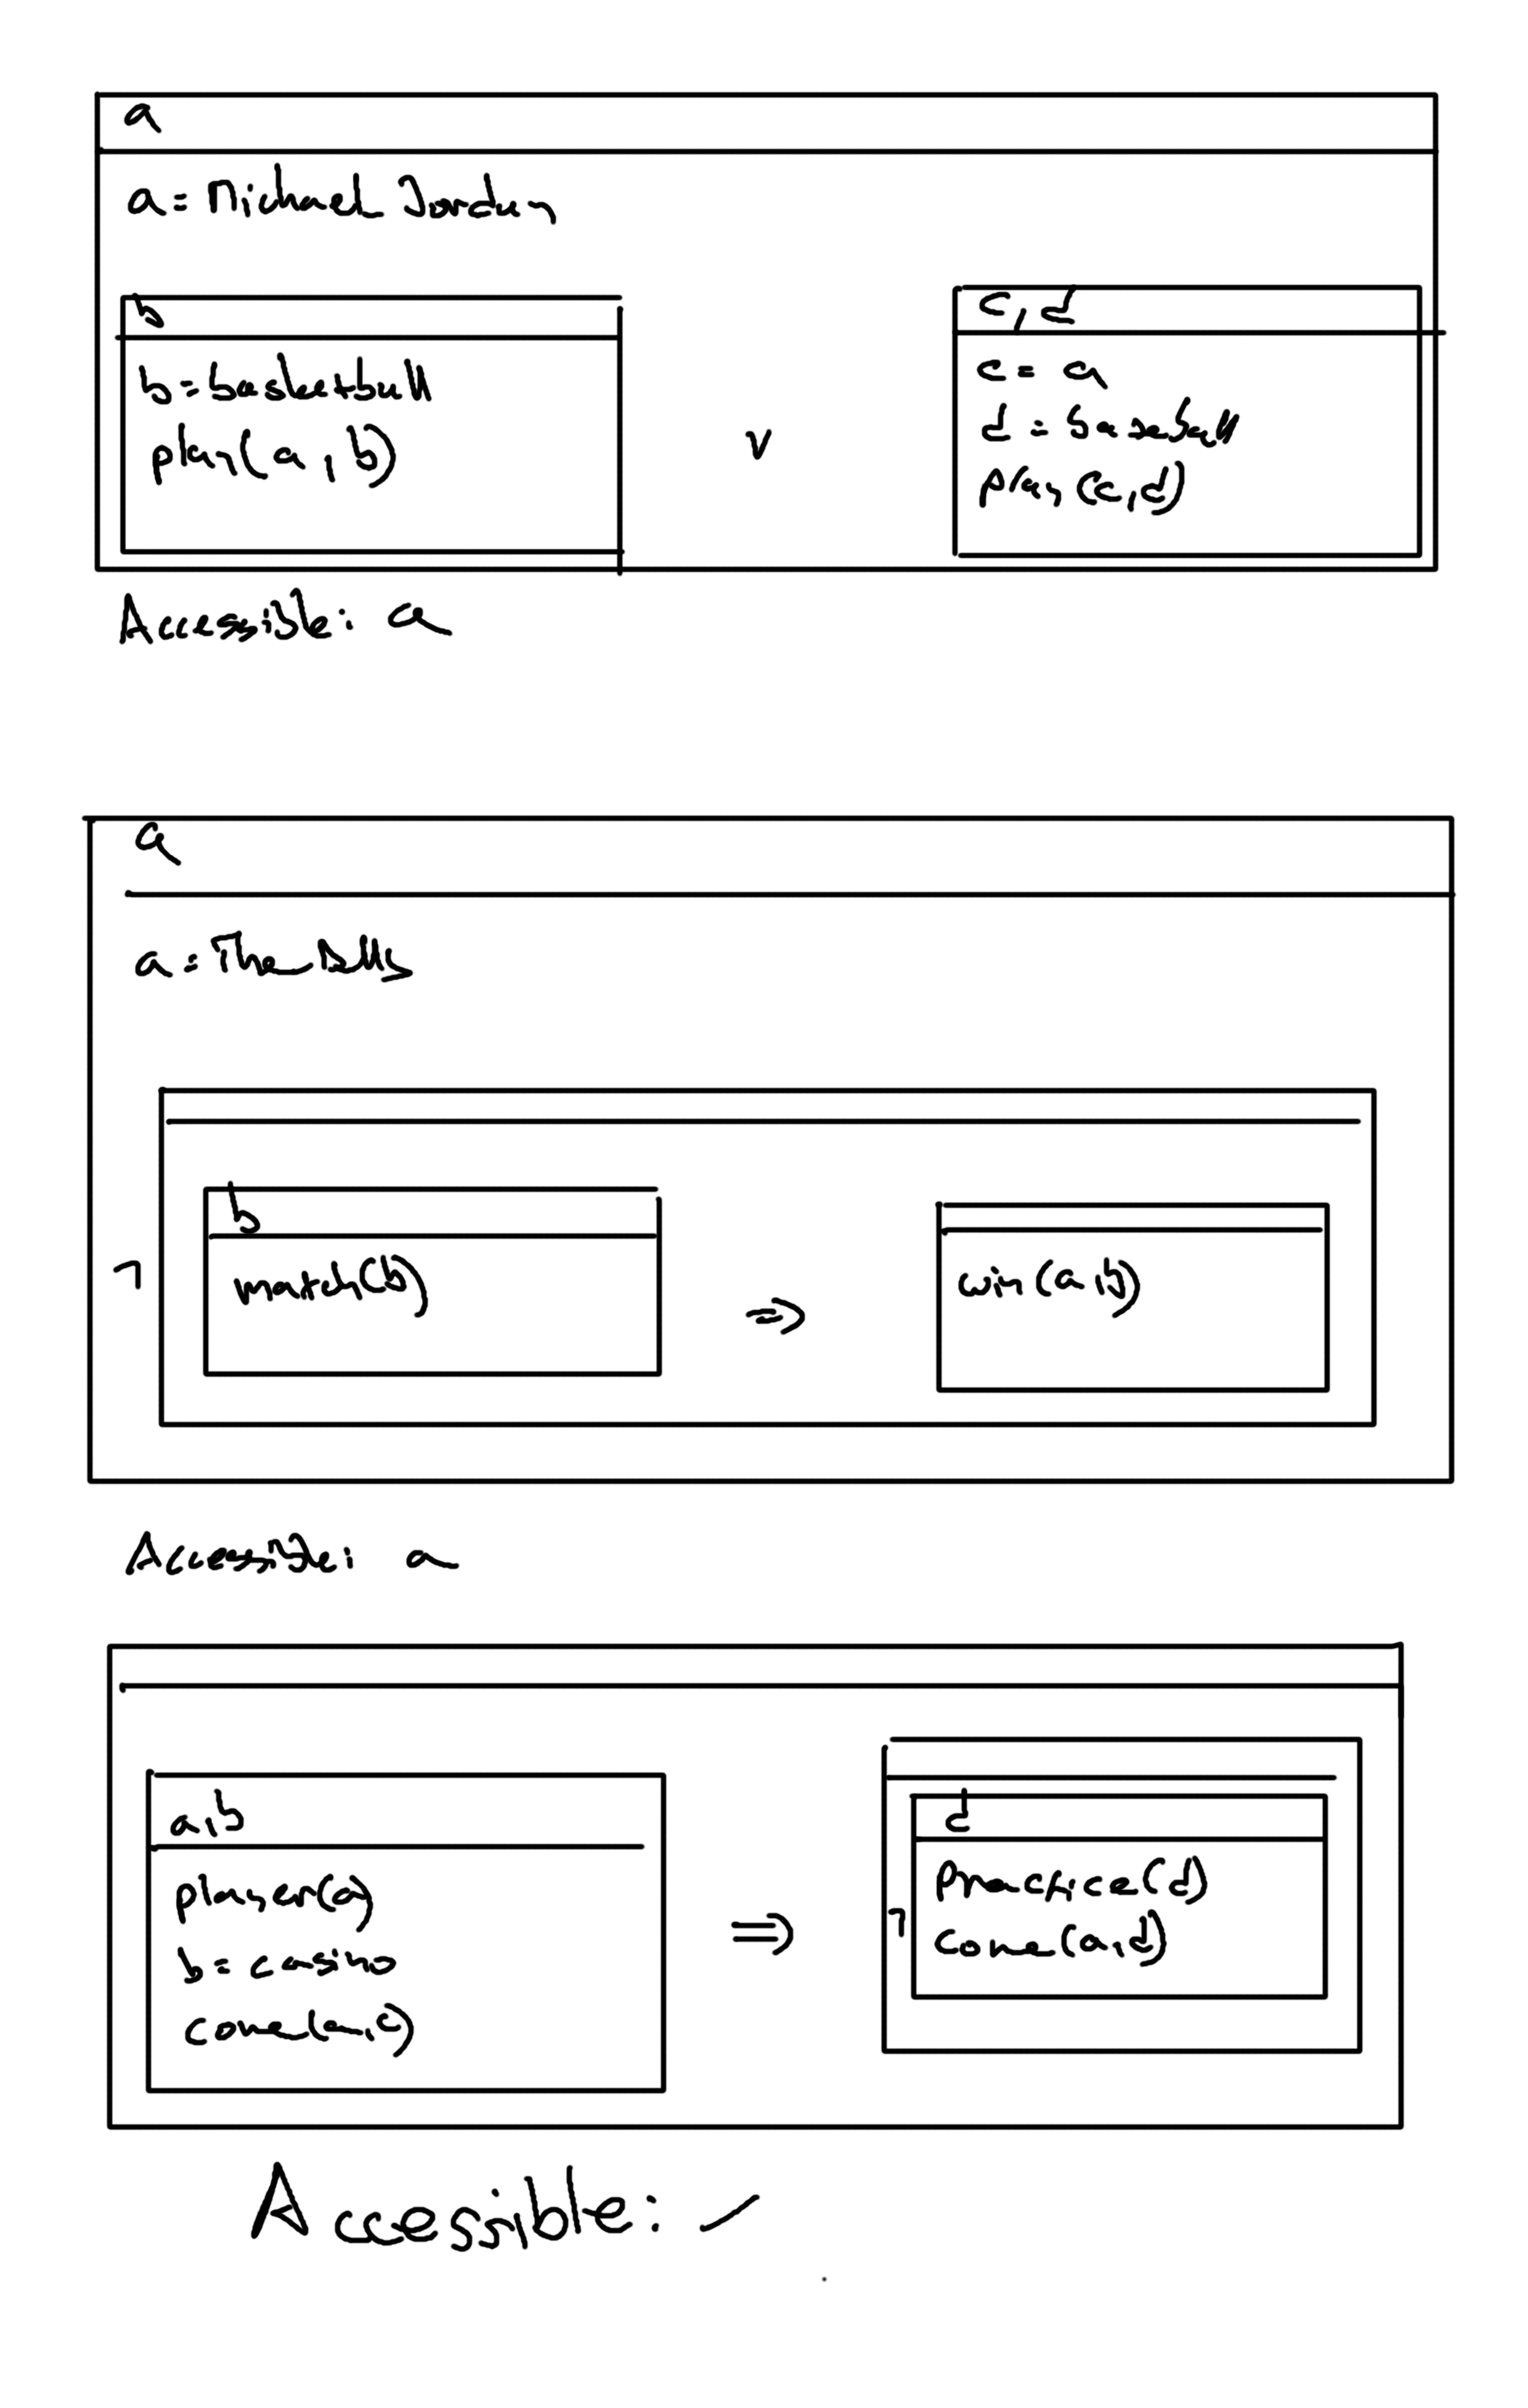
\includegraphics[width=0.8\linewidth]{semantics.png}

\raggedright
\subsubsection*{Truth-condition derivation}

\begin{gather*}
\ldots \text{ is true in } \langle{} U_M, V_M \rangle{} \text{ iff } \exists f: U_D \rightarrow U_M, a \in \text{Dom}(f) \text{ such that: } \\
f(a) = V_M(\text{Michael Jordan}) \text{ and } \\
\bigg[
\big[ \exists g \supseteq_{\{b\}} g(b) = V_M(\text{basketball}) \wedge \langle{} g(a),g(b) \rangle{} \in V_M(\text{play}) \big] \qquad 
\vee \\
\big[ \exists h \supseteq_{\{c, d\}} h(c) = f(a) \wedge h(d) = V_M(\text{baseball}) \wedge \langle{} h(c),h(d) \rangle{} \in V_M(\text{play}) \big]
\bigg]
\end{gather*}

\section{}

\subsection{}
\subsubsection{}

\begin{gather*}
\lambda y \ [\ \emptyset\ | \lambda x\ [\ \emptyset\ | \text{beat}(x,y) ] ] 
\end{gather*}


\subsubsection{}

\begin{gather*}
\lambda G \ [\ \emptyset\ | \lambda H\ [\ x\ | G(x) \rightarrow \neg [\ \emptyset\ | H(x) ] ] ] 
\end{gather*}


\subsubsection{}

\begin{gather*}
\lambda a \ [\ \emptyset\ | \lambda b\ [\ \emptyset\ | a \leftarrow b  ] ] 
\end{gather*}

From my understanding of natural language, the usage \emph{because} is not only the description of the causal relationship but also assertion that both parts are true.

\subsection{}

\begin{gather*}
\lambda a \ [\ \emptyset\ | \lambda b\ [\ \emptyset\ | a \leftarrow b  ] ] \\
([\ m\ | \text{michel} = m, \text{happy}(m) ]) \\
(
    (\lambda M [\ n \ | m = n, M])
    (
        (\lambda G \ [\ \emptyset\ | \lambda H\ [\ x\ | G(x) \rightarrow \neg [\ \emptyset\ | H(x) ] ] ] )
        (\lambda p \ [ | \text{player}(p) ])
        (
            (\lambda y \ [\ \emptyset\ | \lambda x\ [\ \emptyset\ | \text{beat}(x,y) ] ])
            (n)
        )
    )
)
\end{gather*}

\begin{gather*}
[\ \emptyset\ | \lambda b\ [\ m\ | \text{michel} = m, \text{happy}(m) ]) \leftarrow b  ] \\
(
    (\lambda M [\ n \ | m = n, M])
    (
        (\lambda G \ [\ \emptyset\ | \lambda H\ [\ x\ | G(x) \rightarrow \neg [\ \emptyset\ | H(x) ] ] ] )
        (\lambda p \ [ | \text{player}(p) ])
        (\lambda x\ [\ \emptyset\ | \text{beat}(x,n) ])
    )
)
\end{gather*}


\begin{gather*}
[\ \emptyset\ | \lambda b\ [\ m\ | \text{michel} = m, \text{happy}(m) ]) \leftarrow b  ] \\
(
    (\lambda M [\ n \ | m = n, M])
    ([\ x\ | \text{player}(x) \rightarrow \neg [\ \emptyset\ | \text{beat}(x,n) ])
)
\end{gather*}

\begin{gather*}
[\ \emptyset\ | \lambda b\ [\ m\ | \text{michel} = m, \text{happy}(m) ]) \rightarrow b  ] \\
(
    [\ n \ | m = n, [\ x\ | \text{player}(x) \rightarrow \neg [\ \emptyset\ | \text{beat}(x,n) ]]
)
\end{gather*}

\begin{gather*}
[\ m\ | \text{michel} = m, \text{happy}(m)) \leftarrow [\ n \ | m = n, [\ x\ | \text{player}(x) \rightarrow \neg [\ \emptyset\ | \text{beat}(x,n) ]]]]
\end{gather*}

\end{document}
